\section{Evaluation}
\label{sec:eval}

\sloppy{}
The evaluation will answer the following research questions in order as follows. 

\begin{itemize}
\item What is the performance overhead of \cheetah{}? (\ref{sec:perf})

\item How effective can \cheetah{} detect false sharing problems? How helpful are outputs in fixing false sharing problems?  (\ref{sec:effectiveness})

\item How is the precision of assessment on each false sharing instance?  (\ref{sec:precision})

\end{itemize}

\paragraph{Experimental Setup.} We evaluate \cheetah{} on an AMD Opteron machine, which has 48 1.6 GHz cores, 64 KB private L1 data cache, 512 KB private L2 cache, 10 MB shared L3 cache, and 128 GB memory. We use gcc-4.6 with {\tt -O2} option to compile all applications. Since the machine is a NUMA machine and the performance may vary with different scheduling policy, we bind the threads to cores for the purpose of consistent performance.   

\paragraph{Evaluated Applications.} As prior work~\cite{Sheriff, Predator, qinzhao, mldetect}, we perform experiments on two well-known benchmark suites, Phoenix~\cite{phoenix-hpca} and PARSEC~\cite{parsec}. We intentionally use 16 threads in order to run applications a little longer, since \cheetah{} needs enough samples to detect false sharing problems. If that is still not enough, we change the source code by adding a loop or use a larger input so that every benchmark will run at least 5 seconds to collect enough samples.

\subsection{Performance Overhead}
\label{sec:perf}

\begin{figure*}[htbp]
\centering
\label{fig:overhead}
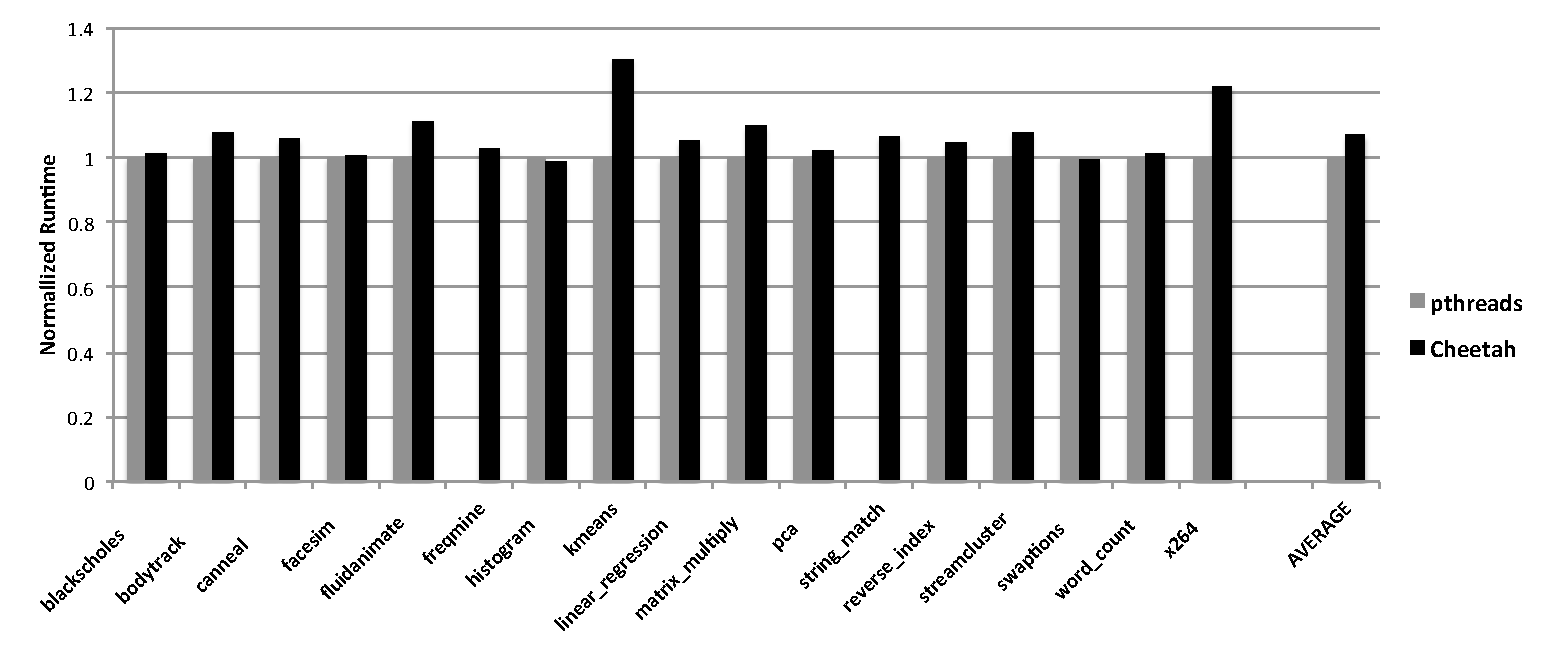
\includegraphics[width=2\columnwidth]{figure/Overhead.pdf}
\caption{Runtime overhead of \Cheetah{}. We normalize the runtime to that of \pthreads{}. On average, \cheetah{} only introduces around 7\% performance overhead on all evaluated benchmarks, which makes it practical to be used in the deployed software. }
\end{figure*}

We show the average runtime overhead of \cheetah{} in Figure~\ref{fig:overhead}. We run each application for five times and show the average results here. According to this figure, \cheetah{} only introduces around 7\% performance overhead, which makes it practical to be utilized in the real deployment. 

During the evaluation, we configure \cheetah{} with the sampling frequency at 64K instructions. Thus, for every 64K instructions, the trap handler will be notified once so that \cheetah{} can collect the information of each sampled memory access. Because of \cheetah{}'s very coarse sampling rate, we should let programs to run sufficiently long enough. 

The performance overhead of \cheetah{} mainly comes from every sampled memory access and each thread creation. For each sampled access, we will collect information such as the type of access (read or write), the number of cycles, and update corresponding data structure such as the history table of its cache line. \cheetah{} also intercepts every thread creation to setup the PMU unit, get the timestamp and update the phase information. The setting of the PMU registers introduces non-negligible overhead since it invokes six pfmon APIs and six additional system calls. For applications with a big number of threads, including \texttt{kmeans} (with 224 threads, running around 14 seconds) and \texttt{x264} (with 1024 threads, running around 40 seconds), we observe that \cheetah{} introduces significantly higher performance overhead than other threads. For other applications, \cheetah{} introduces less than 12\% performance overhead, with 4\% overhead on average if these two applications are excluded.  

%\todo{Check the creation of threads for kmeans and x264. Initializing IBS registers for every thread adds significant performance overhead. Kmeans 224 threads in 14 seconds. 1023 threads in 40 seconds.  }

%\todo{Should we check how the performance overhead will be changed at a different sample frequency?}
 
\subsection{Effectiveness}
\label{sec:effectiveness}

%The state-of-the-art tool Predator reports five false sharing instances in Phoenix and Parsec benchmark suite, including \texttt{histogram}, \texttt{linear\_regression}, \texttt{reverse\_index}, \texttt{streamcluster}, and \texttt{word\_count}~\cite{Predator}. 
\cheetah{} successfully detects two known false sharing problems with significant performance impact, including\texttt{linear\_regression} in Phoenix and \texttt{streamcluster} in Parsec. 

%In the remaining of this section, we discuss how reported information can help us to confirm and fix these false sharing problems. 

%Finally, we study the false sharing that \cheetah{} does not detect in these benchmarks and verify that they have negligible impact to the overall program execution. 

\subsubsection{Case Study: linear\_regression}
Figure~\ref{fig:lr} shows the output of \cheetah{}. It points out that the {\tt tid\_args} object allocated at line 139, with the structure type {\tt lreg\_args}, incurs a severe false sharing problem. According to the assessment, fixing it can possibly improve the performance by $5.7\times$. By examining the source code, we can discover that the {\tt tid\_args} object is passed to different threads--linear\_regression\_pthread. Then we can easily find out where false sharing has been exercised, which is shown as Figure~\ref{lr:code}. By checking the word-based accesses that is not shown here, we can understand the reason of this false sharing problem: different threads are updating different parts of the object {\tt tid\_args} simultaneously, where each thread updates the size of the structure lreg\_args of this common array. This problem is similar to the example shown in Figure~\ref{fig:penalty}. 

To address the problem, we pad the structure {\tt lreg\_args} with extra bytes, by adding 64 bytes useless content, so that we can force different threads not to access the same cache line. The simple optimization lead to a 5.7$\times$ speedup, which matches the assessment 5.76$\times$ predicted by \cheetah{}.

\begin{figure}
\begin{minipage}{\columnwidth}

\centering

\fbox
{
%\scriptsize
\begin{minipage}{3in}
Detecting false sharing at the object: start 0x400004b8 end 0x400044b8 (with size 4000). \\
Accesses 1263 invalidations 27f writes 501 total latency 102988 cycles.\\
\\
Latency information: \\
totalThreads 16 \\
totalThreadsAccesses 12e1 \\
totalThreadsCycles 106389 \\
%longestRuntime 7652 \\
%threadReduceRate 0.164697 \\
totalPossibleImprovementRate 576.172748\% \\
(realRuntime 7738 predictedRuntime 1343).\\
\\
It is a heap object with the following callsite:\\
linear\_regression-pthread.c: 139
\end{minipage}
}
\vspace{1em}
\caption{\cheetah{} reports a false sharing problem in \texttt{linear\_regression}.}
\label{fig:lr}
\end{minipage}
\end{figure}


\begin{figure}
%\scriptsize
\begin{verbatim}
typedef struct
{
  ......  
  long long SX;
  long long SY;
  long long SXX;
  ......
} lreg_args;	

for (i = 0; i < args->num_elems; i++)
{
  //Compute SX, SY, SYY, SXX, SXY
  args->SX  += args->points[i].x;
  args->SXX += args->points[i].x
              *args->points[i].x;
  args->SY  += args->points[i].y;
  ......
}
\end{verbatim}
\caption{The data structure and source code related to a serious false sharing instance in \texttt{linear\_regression}.}
\label{lr:code}
\end{figure}

\subsubsection{Case Study: streamcluster}

%Figure~\ref{fig:sc} shows the output of StreamCluster. 
We do not show the report results of streamcluster because of space limit. For streamcluster, every thread will update the work\_mem object concurrently, allocated at line 985 of the \texttt{streamcluster.cpp} file. The authors have already added some padding to avoid false sharing. However, the size of cache line (as a macro) is set to be 32 bytes, which is smaller than the size of actual cache line used in our experimental machine. Thus, streamcluster will still has a significant false sharing problem. The performance impact of fixing false sharing problems inside is further discussed in Section~\ref{sec:precision}. 


\subsubsection{Comparing with State-of-the-art}

\begin{figure}[htbp]
\centering
\label{fig:fseffectiveness}
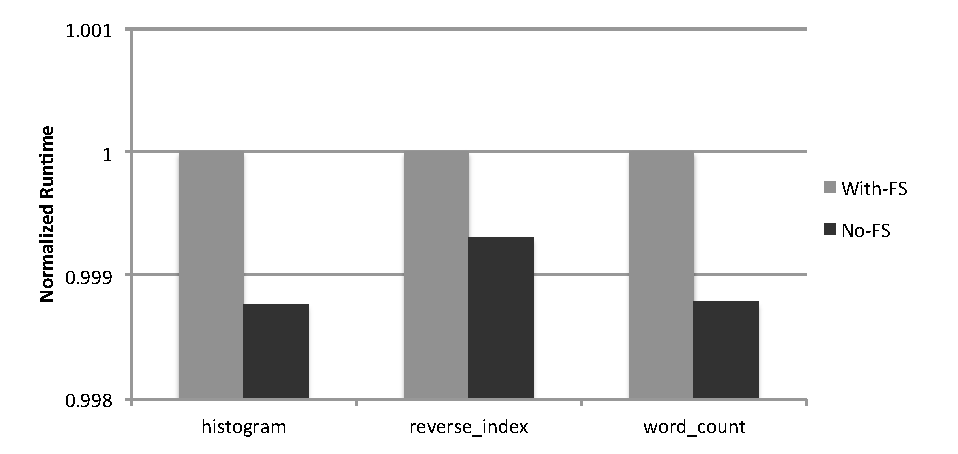
\includegraphics[width=.9\columnwidth]{figure/trivial.pdf}
\caption{False sharing problems missed by \cheetah{} have negligible (<0.2\%) performance impact .}
\end{figure}

%\cheetah{} may miss some false sharing instances because of its sampling feature. 
As discussed before, \cheetah{} only detects false sharing problems that actually occur in the execution and can have significant performance impact on the final performance. As observed by Predator~\cite{Predator}, the occurrences of false sharing can be affected by the starting address of objects or the size of the cache line. The performance impact of a false sharing can be greatly impacted by the cache hierarchy. If the number of accesses on a falsely-shared object is not large enough, \cheetah{} may not be able to detect it because of its sampling feature. 

%. In this section, we will compare \cheetah{}'s effectiveness with the state-of-the-art tool -- Predator~\cite{Predator}, which observes the largest number of false sharing instances. 
Comparing with the state-of-the-art tool--Predator, \cheetah{} misses false sharing problems in  \texttt{histogram}, \texttt{reverse\_index} and \texttt{word\_count}~\cite{Predator}. We further fix these false sharing problems according to Predator's detection results. We run these applications on our experimental hardware, with and without false sharing problems. Figure~\ref{fig:fseffectiveness} shows the performance impact. According to Figure~\ref{fig:fseffectiveness}, all of these benchmarks do not show a significant speedup after fixing, with less than 0.2\% performance improvement. This behavior actually exemplifies the advantage of \Cheetah{}: \emph{since \cheetah{} only reports false sharing problems with significant performance impact, it can potentially save programmers manual effort unnecessarily spending on applications with trivial performance improvement}. 

\subsection{Assessment Precision}
\label{sec:precision}

Different with all existing tools, \cheetah{} is the first tool that can assess the performance impact of false sharing problems. This section evaluates the precision of assessment. 

We evaluate the precision of assessment on two applications, \texttt{linear\_regression} and \texttt{streamcluster}, since they are observed to have serious false sharing problems. We listed the results in Table~\ref{tbl: precision}. In this table, \texttt{linear\_regression} is abbreviated as ``linear\_reg''.  We evaluate these two applications when the number of threads is equal to 16, 8, 4, and 2 correspondingly. We list the predicted performance impact in the ``Predict'' column and the actual improvement in the ``Real'' column of the table. The last column (``Diff'') of this table lists the difference between the predicted improvement and the real improvement. If the number is larger than 0, the predicted performance improvement is less than the real improvement. Otherwise, it is the opposite. 
%The difference is calculated by dividing the difference by the real improvement.  

Table~\ref{tbl: precision} shows that \cheetah{} can perfectly assess the performance impact of false sharing in every case, with less than 10\% difference for every evaluated execution. %Relying on the assessment, programmers do not have to spend time on trivial false sharing problems any more. 
\emph{According to this novel assessment of \cheetah{}, programmers may save huge amount of manual effort spending unnecessarily on applications with trivial false sharing problems}. 

\begin{table}
  \small
  \centering
  \begin{tabular}{ c | c | c | c | c}
  \hline
  \textbf{Application} & \specialcell{Threads \\ (\#)} & \textbf{Predict} & \textbf{Real} & \specialcell{Diff \\ (\%)}\\ \hline
\texttt{linear\_reg} & 16 & 6.44X    & 6.7X & {-3.8}\\
\texttt{linear\_reg}& 8  & 5.56X    & 5.4X & {+3.0}\\
\texttt{linear\_reg} & 4  & 3.86X  & 4.1X  & {-5.8}\\
 \texttt{linear\_reg}& 2  & 2.18X  & 2X    & {+9}\\ \hline
 \texttt{streamcluster} & 16 & 1.016X    & 1.015X &  {0}\\
 \texttt{streamcluster} & 8 & 1.017X    & 1.018X & {0}\\
 \texttt{streamcluster} & 4 & 1.024X    & 1.022X & {0}\\
 \texttt{streamcluster} & 2 & 1.033X    & 1.035X & {0}
 %\hline
\end{tabular}
  \caption{
    Precision of assessment. \Cheetah{} implements the first method to accurately predict the performance improvement of fixing an observed false sharing instance. \label{tbl: precision}}
\end{table}

